\documentclass[a4paper, 11pt, portuguese]{article}

% --- PACOTES ESSENCIAIS ---
\usepackage[T1]{fontenc}
\usepackage[utf8]{inputenc} % Codificação do ficheiro
\usepackage{babel}          % Suporte para Português
\usepackage{amsmath}        % Fórmulas matemáticas avançadas
\usepackage{amssymb}        % Símbolos matemáticos
\usepackage{graphicx}       % Inclusão de imagens
\usepackage[
    colorlinks=true,        % Links coloridos em vez de caixas
    linkcolor=blue,         % Cor dos links internos
    citecolor=blue,         % Cor das citações (se usar bib)
    urlcolor=blue           % Cor dos URLs
]{hyperref}                 % Links clicáveis (URLs, referências)
\usepackage{geometry}       % Configuração das margens
\usepackage{booktabs}       % Tabelas com melhor aspeto
\usepackage{listings}       % Blocos de código formatados
\usepackage{xcolor}         % Cores (usado nos listings)
\usepackage{float}          % Controlo mais fino da posição de floats (figuras, tabelas)

% --- CONFIGURAÇÕES ---

% Margens da página
\geometry{
 a4paper,
 margin=2.5cm, % Margem de 2.5cm em todos os lados
}

% Estilo para blocos de código C++
\definecolor{codegray}{rgb}{0.5,0.5,0.5} % Cor para comentários
\definecolor{codeblue}{rgb}{0,0,0.6}    % Cor para palavras-chave
\definecolor{codegreen}{rgb}{0,0.6,0}  % Cor para strings
\lstdefinestyle{cppstyle}{
    language=C++,
    basicstyle=\ttfamily\footnotesize, % Fonte monoespaçada pequena
    commentstyle=\color{codegray}\itshape, % Comentários em cinza itálico
    keywordstyle=\color{codeblue}\bfseries, % Palavras-chave a azul negrito
    stringstyle=\color{codegreen},    % Strings a verde
    numberstyle=\tiny\color{codegray}, % Números de linha pequenos e cinza
    breaklines=true,                  % Quebra de linhas longas
    frame=single,                     % Caixa à volta do código
    captionpos=b,                     % Legenda em baixo
    showstringspaces=false,           % Não mostrar espaços em strings de forma especial
    tabsize=4,                        % Tamanho da tabulação
    numbers=left,                     % Números de linha à esquerda
    stepnumber=1,                     % Numerar todas as linhas
    numbersep=5pt,                    % Espaço entre números e código
    backgroundcolor=\color{white},    % Fundo branco
    % --- Tratamento de caracteres PT ---
    literate={á}{{\'a}}1 {é}{{\'e}}1 {í}{{\'i}}1 {ó}{{\'o}}1 {ú}{{\'u}}1
             {Á}{{\'A}}1 {É}{{\'E}}1 {Í}{{\'I}}1 {Ó}{{\'O}}1 {Ú}{{\'U}}1
             {â}{{\^a}}1 {ê}{{\^e}}1 {ô}{{\^o}}1
             {Â}{{\^A}}1 {Ê}{{\^E}}1 {Ô}{{\^O}}1
             {ã}{{\~a}}1 {õ}{{\~o}}1
             {Ã}{{\~A}}1 {Õ}{{\~O}}1
             {ç}{{\c{c}}}1 {Ç}{{\c{C}}}1,
}
\lstset{style=cppstyle} % Define o estilo C++ como padrão para listings

% Configuração do idioma principal do documento
\selectlanguage{portuguese}

% --- INFORMAÇÕES DO DOCUMENTO ---
\title{
    
\includegraphics[width=0.4\textwidth]{imagens/ua.pdf} \\ \vspace{1.5cm}
    \textbf{Relatório do Trabalho Laboratorial nº 2} \\
    \large Informação e Codificação (2025/26)
}
\author{
    \textbf{Pedro Miguel Miranda de Melo} (114208) \\
    \textbf{Nome do Aluno 2} (Número Mec.) \\
    \textbf{Nome do Aluno 3} (Número Mec.) \\
    % Adicionar mais linhas conforme necessário
    \textit{Departamento de Eletrónica, Telecomunicações e Informática (DETI)} \\
    \textit{Universidade de Aveiro}
}
\date{Novembro de 2025}

% --- INÍCIO DO DOCUMENTO ---
\begin{document}

\maketitle
\thispagestyle{empty} % Remove número de página na folha de rosto

\newpage
\tableofcontents % Gera o índice automaticamente
\newpage

% ----------------------------------------------------------------------------------
% SECÇÃO 1: INTRODUÇÃO
% ----------------------------------------------------------------------------------
\section{Introdução}

Este relatório documenta o desenvolvimento e os resultados obtidos no âmbito do Trabalho Laboratorial nº 2 da unidade curricular de Informação e Codificação (2025/26), lecionada no Departamento de Eletrónica, Telecomunicações e Informática (DETI) da Universidade de Aveiro.

O projeto foca-se em duas áreas principais: a manipulação básica de imagens digitais utilizando a biblioteca OpenCV e a implementação de um sistema de codificação entrópica (Codificação Golomb) aplicado à compressão sem perdas (\textit{lossless}) de sinais de áudio e imagem. O desenvolvimento foi realizado em C/C++, complementando as ferramentas desenvolvidas no trabalho anterior com novas funcionalidades.

O código-fonte completo do projeto está disponível publicamente no seguinte repositório GitHub: \url{https://github.com/Rubenc1234/IC_miniP1/tree/main/Project2}.

% ----------------------------------------------------------------------------------
% SECÇÃO 2: PARTE I - MANIPULAÇÃO DE IMAGENS COM OPENCV
% ----------------------------------------------------------------------------------
\section{Parte I: Manipulação Básica de Imagens com OpenCV}

A primeira parte do trabalho consistiu na familiarização com a biblioteca OpenCV através da implementação de programas para realizar operações fundamentais em imagens digitais, manipulando diretamente os seus píxeis. Foi instalada a versão 4.x da biblioteca, utilizando os pacotes pré-compilados disponíveis através do gestor de pacotes APT (`sudo apt install libopencv-dev pkg-config`).

\subsection{Programa \texttt{extract\_channel}}

Este programa tem como objetivo extrair um canal de cor específico (Azul, Verde ou Vermelho) de uma imagem de entrada, gerando uma imagem de saída em tons de cinza correspondente a esse canal.

\subsubsection{Funcionalidade e Utilização}
O programa lê uma imagem a cores (representada internamente em formato BGR pelo OpenCV). De seguida, cria uma nova imagem monocromática (\texttt{CV\_8UC1}) com as mesmas dimensões. Percorrendo a imagem original píxel a píxel, o valor do canal especificado pelo utilizador (0 para Azul, 1 para Verde, 2 para Vermelho) é copiado para a posição correspondente na imagem de saída. A leitura e escrita dos píxeis é feita usando o método \texttt{Mat::at<>()}.

A sintaxe de utilização é a seguinte:
\begin{lstlisting}[language=bash, caption=Sintaxe de Uso do extract\_channel]
./bin/extract_channel <imagem_entrada> <imagem_saida> <numero_canal>
\end{lstlisting}
Onde \texttt{numero\_canal} deve ser 0, 1 ou 2. O formato da imagem de saída deve ser um que suporte imagens monocromáticas, como \texttt{.pgm} ou \texttt{.png}.

\paragraph{Exemplo de Teste:}
Para extrair os canais Azul (0), Verde (1) e Vermelho (2) da imagem \texttt{airplane.ppm}:
\begin{lstlisting}[language=bash]
./bin/extract_channel img/airplane.ppm imagens/airplane_extract_0.png 0
./bin/extract_channel img/airplane.ppm imagens/airplane_extract_1.png 1
./bin/extract_channel img/airplane.ppm imagens/airplane_extract_2.png 2
\end{lstlisting}

A Figura~\ref{fig:canais_extraidos} mostra o resultado da extração dos três canais de cor.

\begin{figure}[htbp]
\centering
\begin{minipage}{0.48\textwidth}
    \centering
    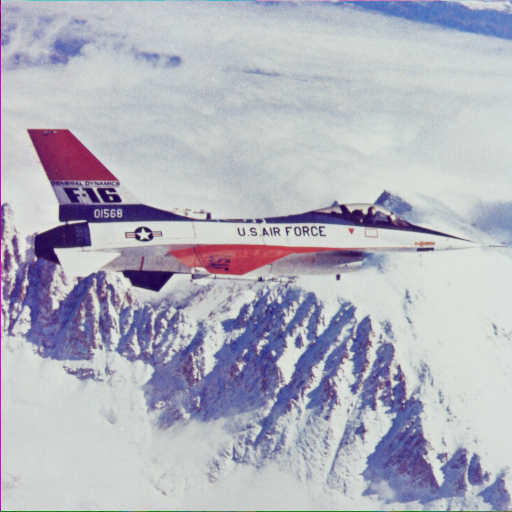
\includegraphics[width=0.8\textwidth]{imagens/airplane.png} % Assumindo que tem uma versão png da original
    \caption*{Imagem Original (airplane)}
\end{minipage}
\hfill
\begin{minipage}{0.48\textwidth}
    \centering
    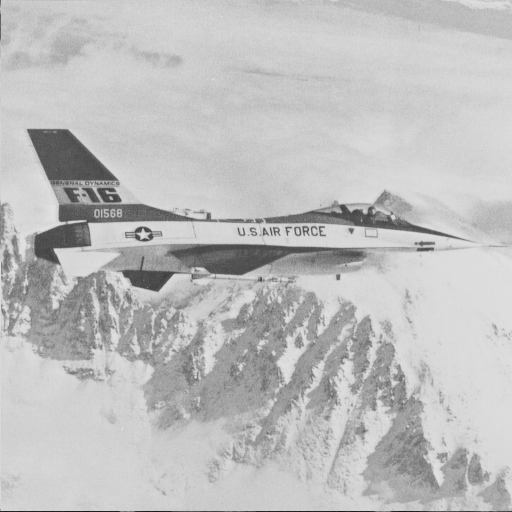
\includegraphics[width=0.8\textwidth]{imagens/airplane_extract_0.png}
    \caption*{Canal Azul (0)}
\end{minipage}
\vspace{0.5cm} % Espaço vertical entre as linhas de imagens
\begin{minipage}{0.48\textwidth}
    \centering
    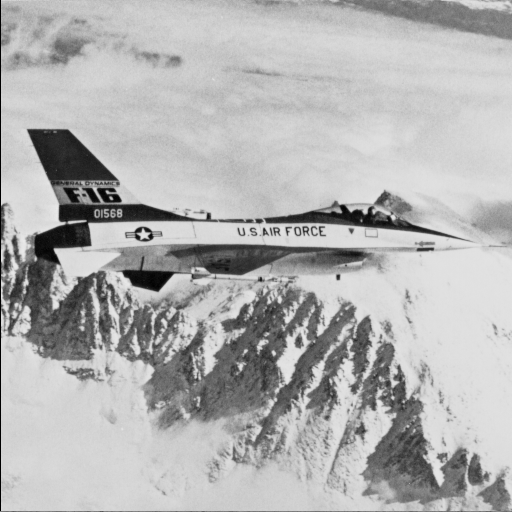
\includegraphics[width=0.8\textwidth]{imagens/airplane_extract_1.png}
    \caption*{Canal Verde (1)}
\end{minipage}
\hfill
\begin{minipage}{0.48\textwidth}
    \centering
    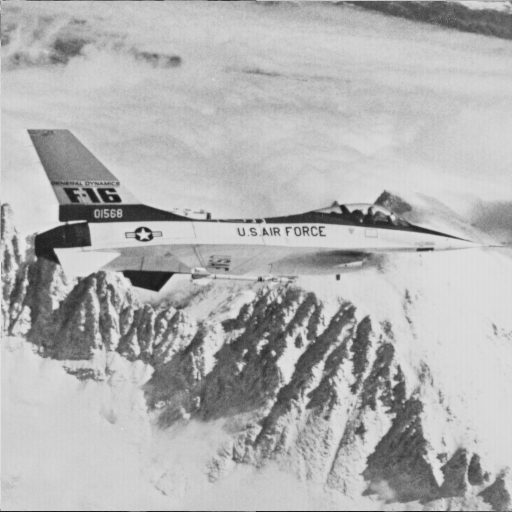
\includegraphics[width=0.8\textwidth]{imagens/airplane_extract_2.png}
    \caption*{Canal Vermelho (2)}
\end{minipage}
\caption{Extração dos canais B, G, R da imagem original.}
\label{fig:canais_extraidos}
\end{figure}

\subsection{Programa \texttt{image\_operations}}

Este programa engloba um conjunto de operações geométricas e de intensidade sobre imagens, implementadas através da manipulação direta dos píxeis, sem recurso a funções específicas do OpenCV para essas transformações. Foram criados executáveis separados para cada operação para maior clareza.

\subsubsection{Negativo da Imagem (\texttt{image\_negative})}
Esta operação inverte os valores de intensidade de cada canal de cor. Para uma imagem de 8 bits por canal, o valor do píxel negativo $P'_{\text{cor}}$ é calculado a partir do original $P_{\text{cor}}$ como:
$$ P'_{\text{cor}} = 255 - P_{\text{cor}} $$
A operação é aplicada independentemente a cada um dos canais B, G, R.

\paragraph{Utilização e Exemplo:}
\begin{lstlisting}[language=bash, caption=Sintaxe de Uso do image\_negative]
./bin/image_negative <imagem_entrada> <imagem_saida> [view]
\end{lstlisting}
\begin{lstlisting}[language=bash]
./bin/image_negative img/airplane.ppm imagens/airplane_neg.png
\end{lstlisting}
O resultado é apresentado na Figura~\ref{fig:negativo}.

\begin{figure}[htbp]
\centering
\begin{minipage}{0.48\textwidth}
    \centering
    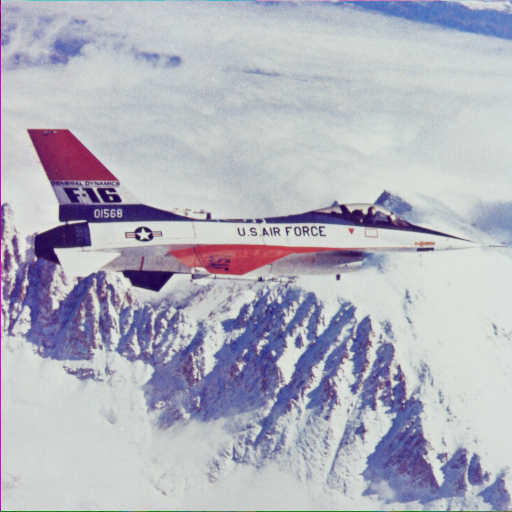
\includegraphics[width=0.8\textwidth]{imagens/airplane.png}
    \caption*{Imagem Original}
\end{minipage}
\hfill
\begin{minipage}{0.48\textwidth}
    \centering
    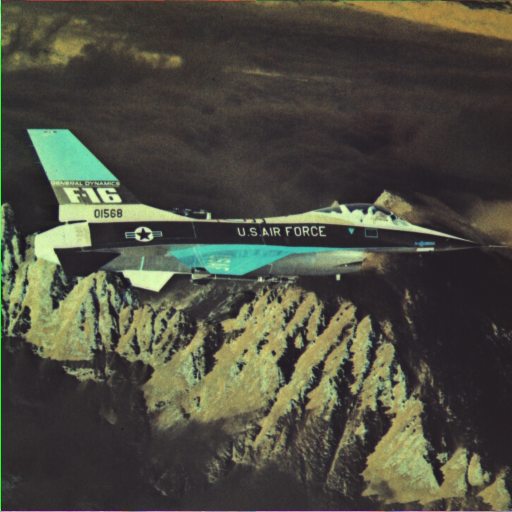
\includegraphics[width=0.8\textwidth]{imagens/airplane_neg.png}
    \caption*{Imagem Negativa}
\end{minipage}
\caption{Resultado da operação de negativo.}
\label{fig:negativo}
\end{figure}

\subsubsection{Espelhamento da Imagem (\texttt{image\_mirror})}
Esta funcionalidade permite espelhar a imagem horizontal ou verticalmente.
\begin{itemize}
    \item \textbf{Espelhamento Horizontal (h):} O píxel $(r, c)$ recebe o valor do píxel $(r, \text{largura} - 1 - c)$.
    \item \textbf{Espelhamento Vertical (v):} O píxel $(r, c)$ recebe o valor do píxel $(\text{altura} - 1 - r, c)$.
\end{itemize}

\paragraph{Utilização e Exemplo:}
\begin{lstlisting}[language=bash, caption=Sintaxe de Uso do image\_mirror]
./bin/image_mirror <imagem_entrada> <imagem_saida> <h | v> [view]
\end{lstlisting}
\begin{lstlisting}[language=bash]
./bin/image_mirror img/airplane.ppm imagens/airplane_mirror_h.png h
./bin/image_mirror img/airplane.ppm imagens/airplane_mirror_v.png v
\end{lstlisting}
Os resultados são apresentados na Figura~\ref{fig:espelhamento}.

\begin{figure}[htbp]
\centering
\begin{minipage}{0.32\textwidth}
    \centering
    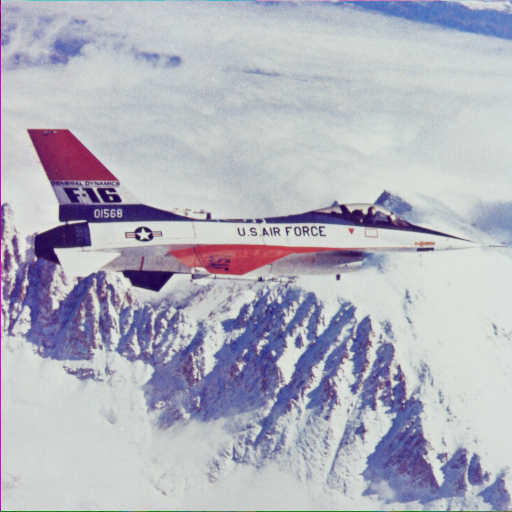
\includegraphics[width=\textwidth]{imagens/airplane.png}
    \caption*{Original}
\end{minipage}
\hfill
\begin{minipage}{0.32\textwidth}
    \centering
    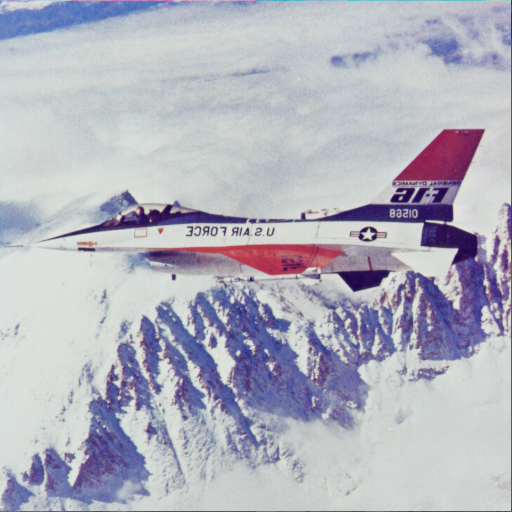
\includegraphics[width=\textwidth]{imagens/airplane_mirror_h.png}
    \caption*{Espelhada Horizontalmente}
\end{minipage}
\hfill
\begin{minipage}{0.32\textwidth}
    \centering
    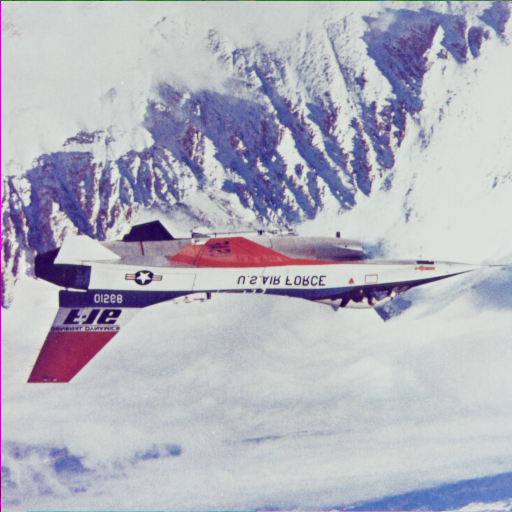
\includegraphics[width=\textwidth]{imagens/airplane_mirror_v.png}
    \caption*{Espelhada Verticalmente}
\end{minipage}
\caption{Resultados da operação de espelhamento.}
\label{fig:espelhamento}
\end{figure}

\subsubsection{Rotação da Imagem (\texttt{image\_rotate})}
Implementa a rotação da imagem por qualquer ângulo múltiplo de 90 graus (positivo, negativo ou zero). O programa normaliza o ângulo fornecido para um equivalente em $\{0, 90, 180, 270\}$ graus no sentido horário e calcula a posição do píxel de origem. Para rotações de 90 ou 270 graus, as dimensões da imagem são trocadas.

\paragraph{Utilização e Exemplo:}
\begin{lstlisting}[language=bash, caption=Sintaxe de Uso do image\_rotate]
./bin/image_rotate <imagem_entrada> <imagem_saida> <angulo>
\end{lstlisting}
\begin{lstlisting}[language=bash]
./bin/image_rotate img/airplane.ppm imagens/airplane_rotated90.png 90
./bin/image_rotate img/airplane.ppm imagens/airplane_rotated180.png 180 % (Gerar esta imagem)
./bin/image_rotate img/airplane.ppm imagens/airplane_rotated270.png 270 % (Gerar esta imagem)
\end{lstlisting}
A Figura~\ref{fig:rotacao} ilustra a rotação de 90 graus.

\begin{figure}[htbp]
\centering
\begin{minipage}{0.48\textwidth}
    \centering
    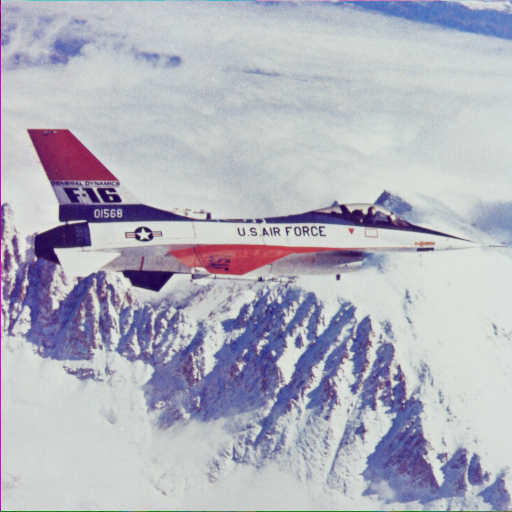
\includegraphics[width=0.7\textwidth]{imagens/airplane.png} % Ajustar tamanho se necessário
    \caption*{Imagem Original}
\end{minipage}
\hfill
\begin{minipage}{0.48\textwidth}
    \centering
    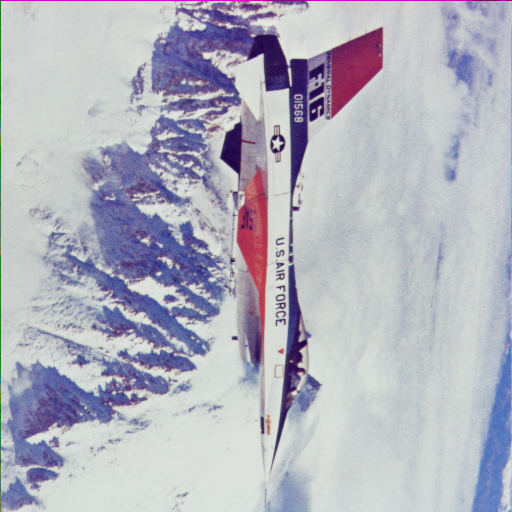
\includegraphics[width=0.7\textwidth]{imagens/airplane_rotated90.png} % angle=-90 para mostrar direita
    \caption*{Rotação 90° Horário}
\end{minipage}
% Adicionar minipages para 180 e 270 se desejar mostrar todas
\caption{Resultado da operação de rotação (exemplo para 90°).}
\label{fig:rotacao}
\end{figure}

\subsubsection{Ajuste de Intensidade (\texttt{image\_intensity})}
Permite aumentar ou diminuir o brilho geral da imagem. O programa aceita um valor percentual no intervalo $[-100, 100]$. Este valor é mapeado para um ajuste aditivo $A$ no intervalo $[-255, 255]$:
$$ A = \text{round}(\text{percentagem} \times 2.55) $$
Este valor $A$ é somado a cada canal de cor (B, G, R) de cada píxel. A função \texttt{saturate\_cast<uchar>} garante que o resultado final permaneça no intervalo válido $[0, 255]$.

\paragraph{Utilização e Exemplo:}
\begin{lstlisting}[language=bash, caption=Sintaxe de Uso do image\_intensity]
./bin/image_intensity <imagem_entrada> <imagem_saida> <percentagem_ajuste>
\end{lstlisting}
\begin{lstlisting}[language=bash]
./bin/image_intensity img/airplane.ppm imagens/airplane_brighter_50.png 50
./bin/image_intensity img/airplane.ppm imagens/airplane_darker_-50.png -50
\end{lstlisting}
A Figura~\ref{fig:intensidade} mostra os resultados para aumento e diminuição de 50\%.

\begin{figure}[htbp]
\centering
\begin{minipage}{0.32\textwidth}
    \centering
    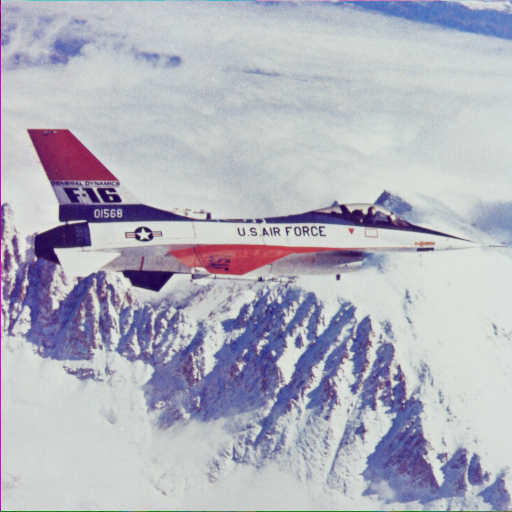
\includegraphics[width=\textwidth]{imagens/airplane.png}
    \caption*{Original (0\%)}
\end{minipage}
\hfill
\begin{minipage}{0.32\textwidth}
    \centering
    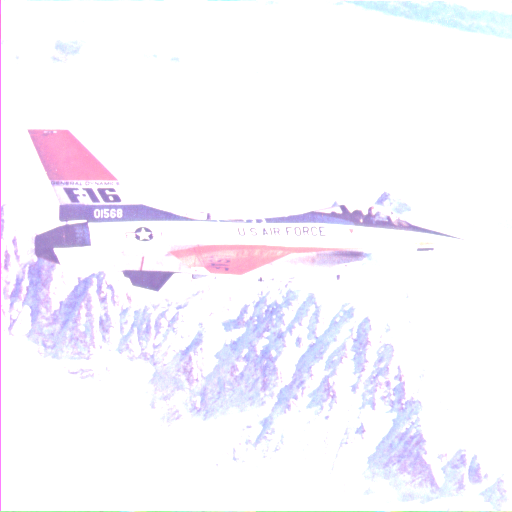
\includegraphics[width=\textwidth]{imagens/airplane_brighter_50.png}
    \caption*{Brilho +50\%}
\end{minipage}
\hfill
\begin{minipage}{0.32\textwidth}
    \centering
    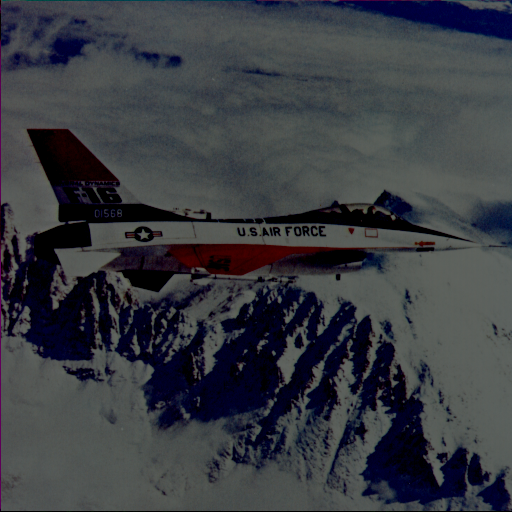
\includegraphics[width=\textwidth]{imagens/airplane_darker_-50.png}
    \caption*{Brilho -50\%}
\end{minipage}
\caption{Resultados da operação de ajuste de intensidade.}
\label{fig:intensidade}
\end{figure}

% ----------------------------------------------------------------------------------
% SECÇÃO 3: PARTE II - CLASSE DE CODIFICAÇÃO GOLOMB
% ----------------------------------------------------------------------------------
\section{Parte II: Classe de Codificação Golomb}

Esta parte focou-se na implementação de uma classe C++ para a codificação Golomb, uma técnica de codificação entrópica eficiente para fontes com distribuições geométricas ou de Laplace.

\subsection{Classe \texttt{GolombCodec}} % (Assumindo este nome para a classe)

% -- Descrever aqui a classe GolombCodec --
% - Construtor (parâmetro m)
% - Método encode(int valor) -> devolve sequência de bits (e.g., string ou vector<bool>)
% - Método decode(sequência de bits) -> devolve int
% - Tratamento de negativos (Sinal+Magnitude e Interleaving)
% - Explicação da fórmula de codificação/descodificação (quociente unário, resto binário)
% - Como o parâmetro 'm' afeta os códigos


% ----------------------------------------------------------------------------------
% SECÇÃO 4: PARTE III - CODEC ÁUDIO LOSSLESS
% ----------------------------------------------------------------------------------
\section{Parte III: Codec Áudio Lossless}

Nesta secção, foi desenvolvido um codec de áudio sem perdas (\textit{lossless}), utilizando a codificação Golomb implementada na Parte II para comprimir os resíduos de predição.

\subsection{Arquitetura do Codec (\texttt{audio\_golomb\_codec})}

% -- Descrever aqui a arquitetura --
% - Encoder e Decoder
% - Suporte Mono e Estéreo
% - Processamento (amostra a amostra ou bloco a bloco?)
% - Predição Temporal:
%   - Explicar o(s) preditor(es) usados (e.g., P[n] = x[n-1], P[n] = 2x[n-1] - x[n-2], etc.)
%   - Cálculo do resíduo: e[n] = x[n] - P[n]
% - Predição Inter-Canal (para Estéreo):
%   - Explicar como um canal é usado para prever o outro (e.g., L[n] previsto por R[n], ou vice-versa, ou usando MID/SIDE?)
%   - Como os resíduos dos dois canais são tratados/codificados
% - Codificação Golomb dos Resíduos:
%   - Como o parâmetro 'm' é tratado (Fixo? Adaptativo?)
%   - Como os números negativos (resíduos) são tratados (Sinal+Magnitude ou Interleaving?)
% - Formato do Ficheiro Comprimido (Header + Dados Golomb)

\subsection{Análise de Desempenho e Compressão}

% -- Apresentar aqui os resultados --
% - Tabela com taxas de compressão para vários ficheiros de áudio (mono/estéreo)
% - Tabela com tempos de codificação/descodificação
% - Comparação com FLAC (ou outro codec lossless standard)


% ----------------------------------------------------------------------------------
% SECÇÃO 5: PARTE IV - CODEC IMAGEM LOSSLESS (GRAYSCALE)
% ----------------------------------------------------------------------------------
\section{Parte IV: Codec Imagem Lossless (Grayscale)}

Aplicando os mesmos princípios da Parte III, foi desenvolvido um codec sem perdas para imagens em escala de cinza.

\subsection{Arquitetura do Codec (\texttt{image\_golomb\_codec})}

% -- Descrever aqui a arquitetura --
% - Encoder e Decoder
% - Processamento da imagem (pixel a pixel? linha a linha?)
% - Predição Espacial:
%   - Explicar o(s) preditor(es) usados (e.g., P(x,y) = N, P(x,y) = W, P(x,y) = N+W-NW, JPEG-LS MED ou LOCO-I?)
%   - Cálculo do resíduo: e(x,y) = I(x,y) - P(x,y)
% - Codificação Golomb dos Resíduos:
%   - Otimização do parâmetro 'm' (Fixo por blocos? Adaptativo?)
%   - Tratamento de negativos
% - Formato do Ficheiro Comprimido (Header + Dados Golomb)

\subsection{Análise de Desempenho e Compressão}

% -- Apresentar aqui os resultados --
% - Tabela com taxas de compressão para várias imagens grayscale
% - Tabela com tempos de codificação/descodificação
% - Comparação com PNG, JPEG-LS ou WebP Lossless


% ----------------------------------------------------------------------------------
% SECÇÃO 6: CONCLUSÕES
% ----------------------------------------------------------------------------------
\section{Conclusões}

% -- Resumir o trabalho realizado --
% - Principais desafios e sucessos em cada parte.
% - Discussão sobre a eficácia da codificação Golomb e da predição.
% - Comparação com codecs standard e possíveis melhorias futuras.


% --- BIBLIOGRAFIA (Opcional, se citar fontes externas) ---
%\newpage
%\bibliographystyle{plain}
%\bibliography{referencias} % Cria um ficheiro referencias.bib

\end{document}